\section{Systemarchitektur}

SSWIS baut auf ein MVC-Model auf. Die Benutzerinteraktion erfolgt
über das View. Aus View Model werden abhängige Objecte vom Controller in Model überträgt. Das Controller erzeugt View und Modell Objekte, Programmflusssteuerung. Dabei werden das Bussiness Logic vom Model gehalten.

\begin{figure} 
  \centering
     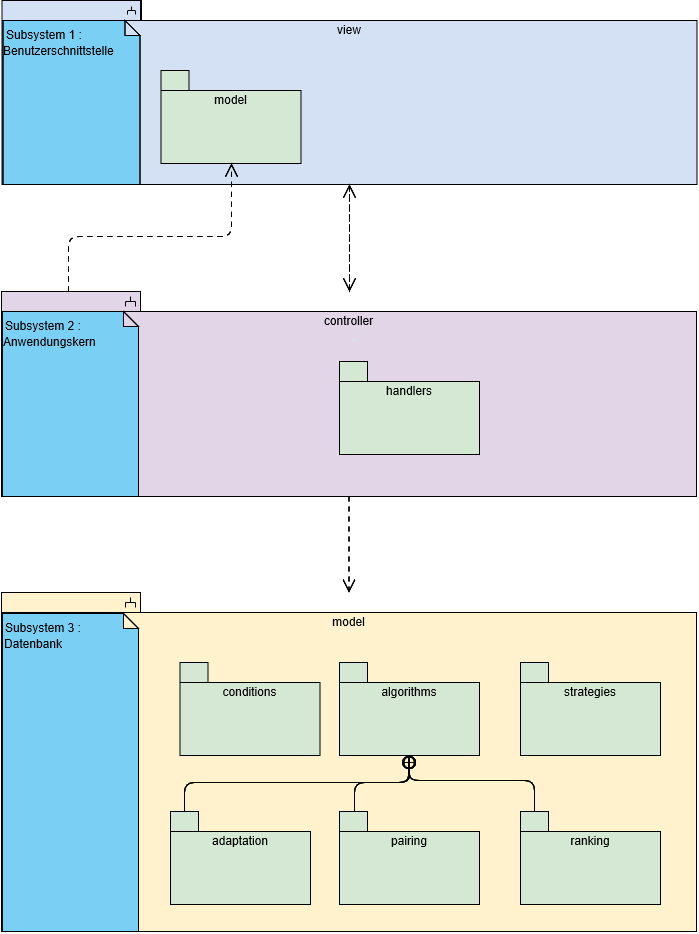
\includegraphics[width=1.1\textwidth]{Systemarchitektur/UMLzuGrobentwurf.png}
\end{figure}

